\section{Parallelization}
\label{sec:md_parallelization}
The parallelization technique is very similar to what we did in DSMC in section \ref{sec:dmsc_parallelization}. The spatial domain is divided into $P_x\times P_y\times P_z$ smaller domains ($P_i$ being the number of processors in the $i$th dimension). Each such domain is then of size $l_x\times l_y \times l_z$ where $l_i = L_i/P_i$. The processor arrangement and labeling is done as shown in figure \ref{fig:md_parallelization_2}, where a processor with coordinates $(p_x, p_y, p_z)$ controls atoms with coordinates in the range
\begin{align}
	\nonumber
	x&\in[p_xl_x, (p_x+1)l_x\rangle\\
	\nonumber
	y&\in[p_yl_y, (p_y+1)l_y\rangle\\
	z&\in[p_zl_z, (p_z+1)l_z\rangle.
\end{align}
\begin{figure}[h!]
\begin{center}
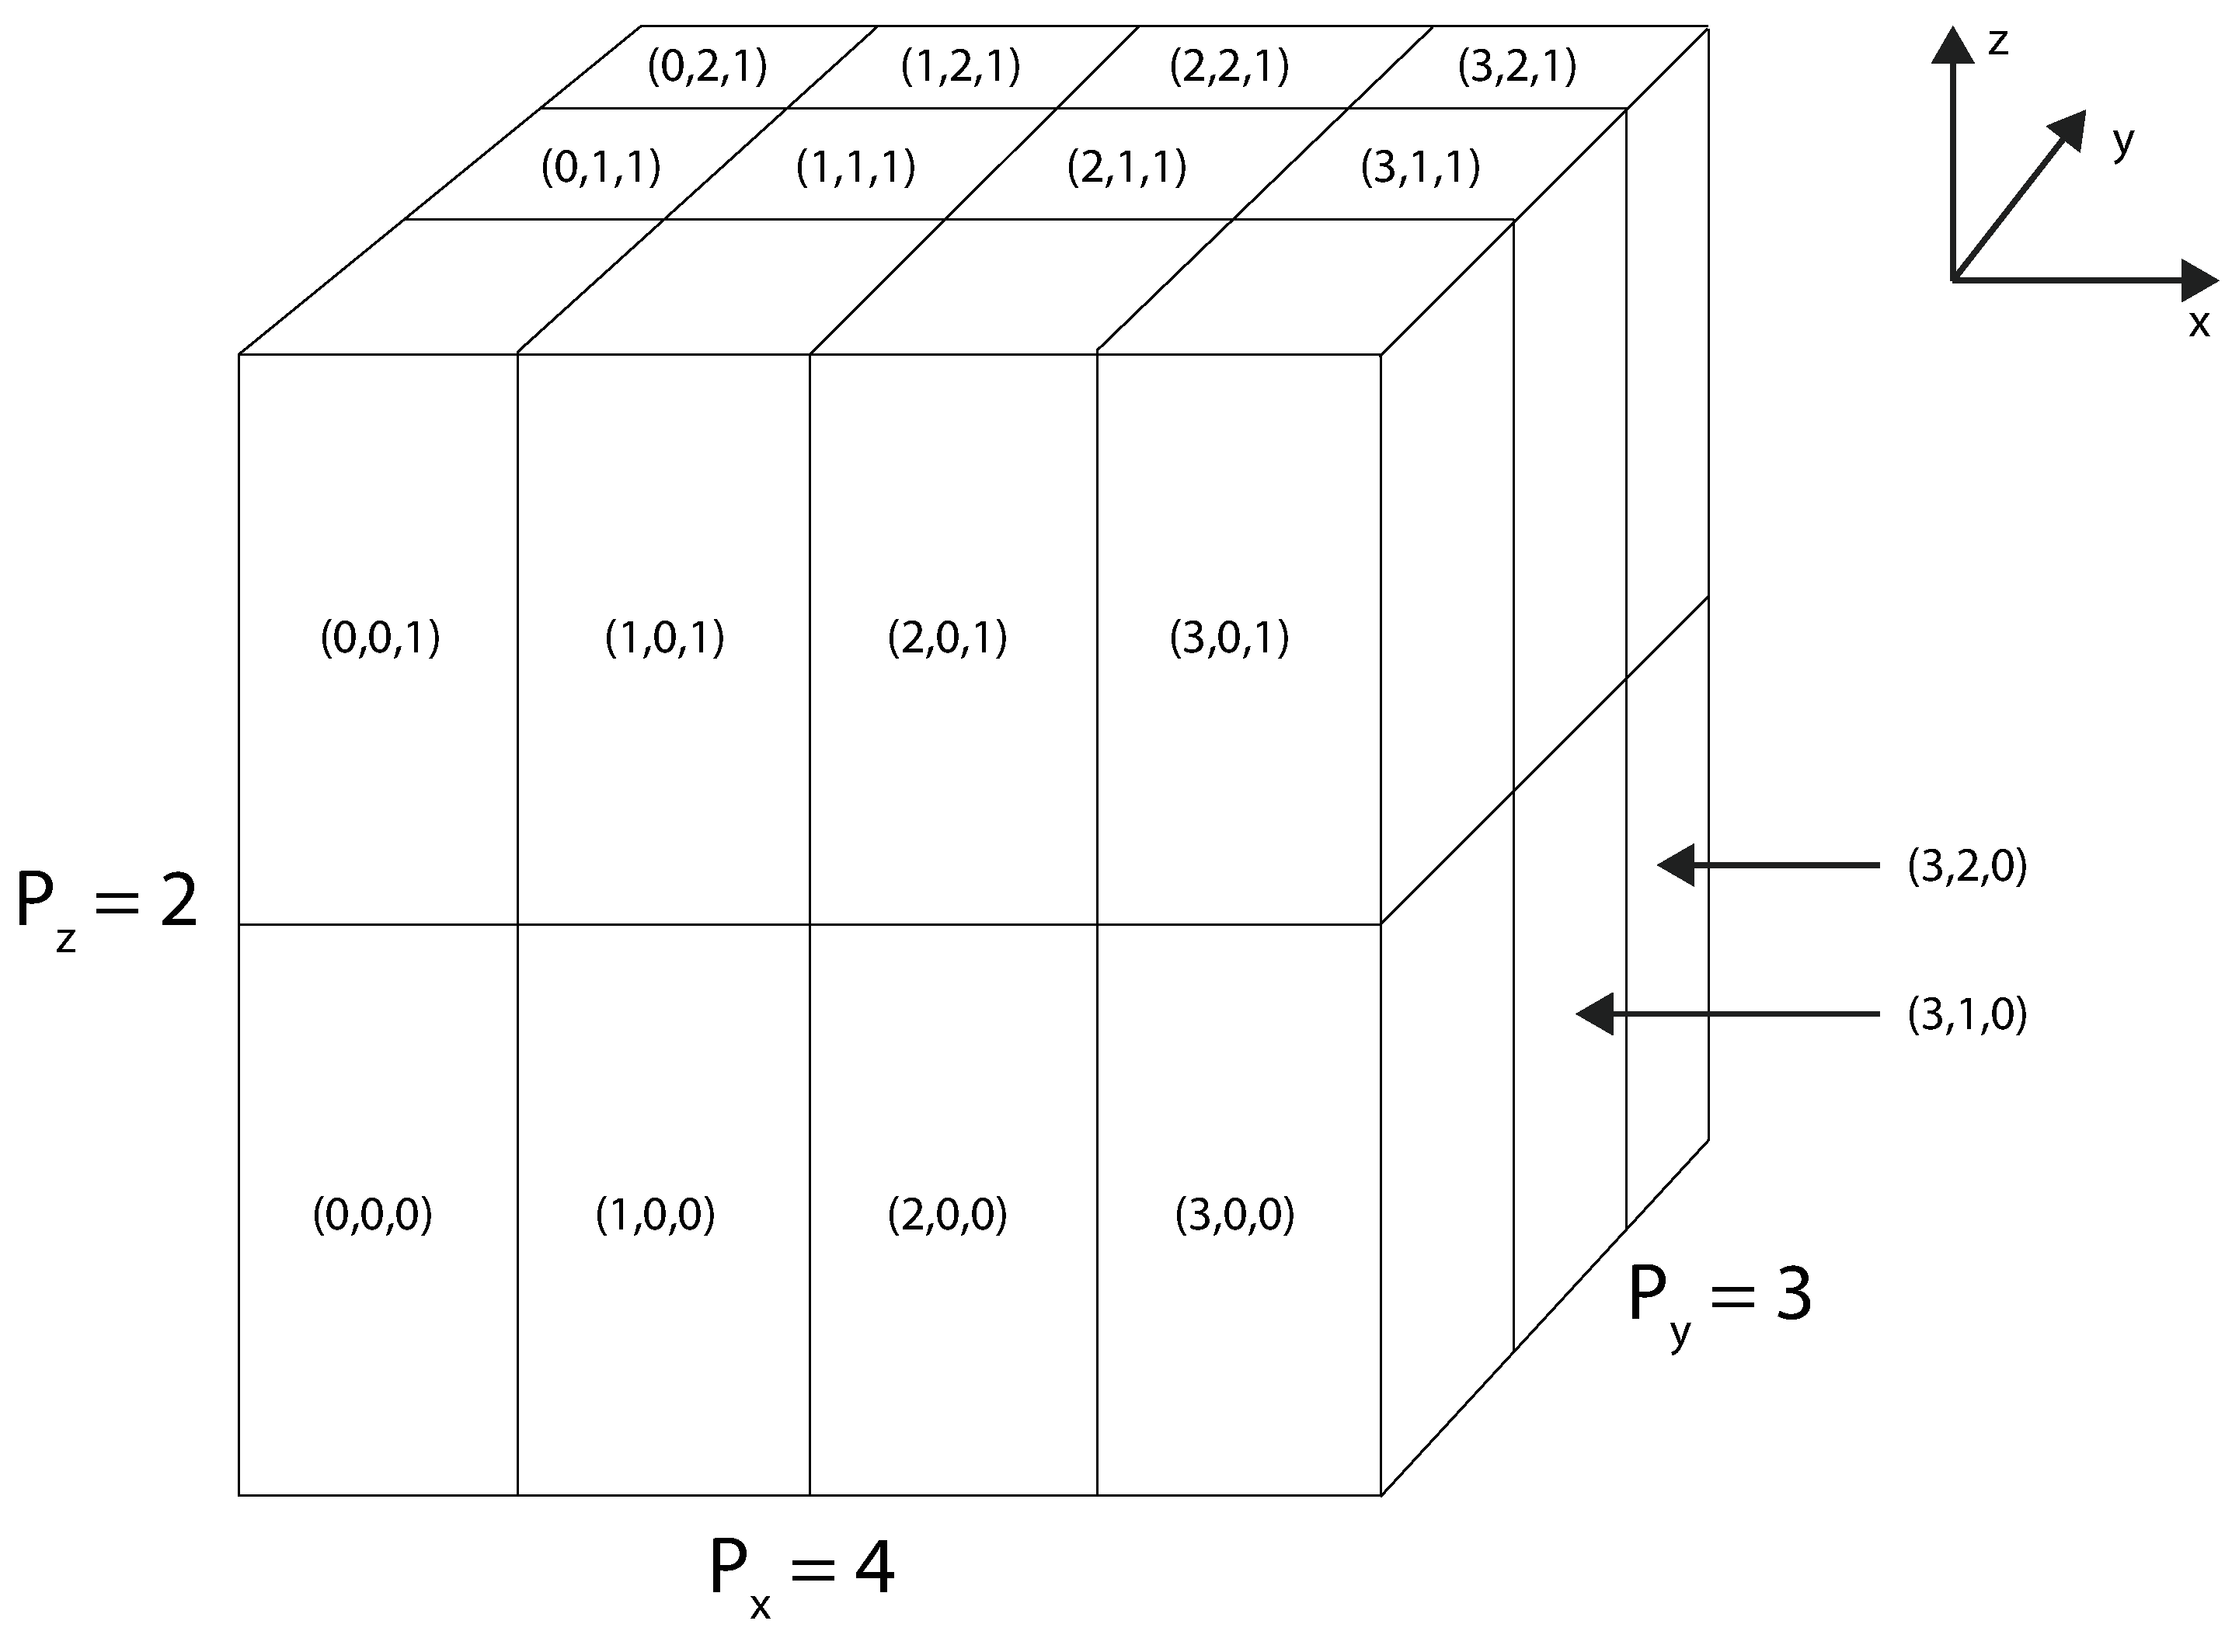
\includegraphics[width=0.7\textwidth, trim=0cm 0cm 0cm 0cm, clip]{DSMC/figures/parallelization_node_configuration.eps}
\end{center}
\caption{Processor labeling in a 3-dimensional grid. Each processor is uniquely identified through its coordinate $(p_x, p_y, p_z)$.}
\label{fig:md_parallelization_2}
\end{figure}
We represent the coordinates of an atom on processor $(p_x, p_y, p_z)$ in the local coordinate system where the CPU's origin $\vec p_\text{origin}$ defines the coordinate system. An atom with global coordinates $\vec r$ will then have local coordinates $\vec r'$
\begin{align}
	\vec r' = \vec r - \vec p_\text{origin}.
\end{align}
We can then easily detect if an atom has moved outside its processor's domain by checking if any of the local coordinate components are outside the range $[0, l_i)$ for dimension $i$. If an atom has moved to another processor, it has moved to one of the 26 neighboring processors. We will use the same 3-step process as described in subsection \ref{sec:dsmc_parallelization_exchange_particles} which is best illustrated with the 2-dimensional example in figure \ref{fig:md_parallelization_facet_technique}.
\begin{figure}[h!]
\begin{center}
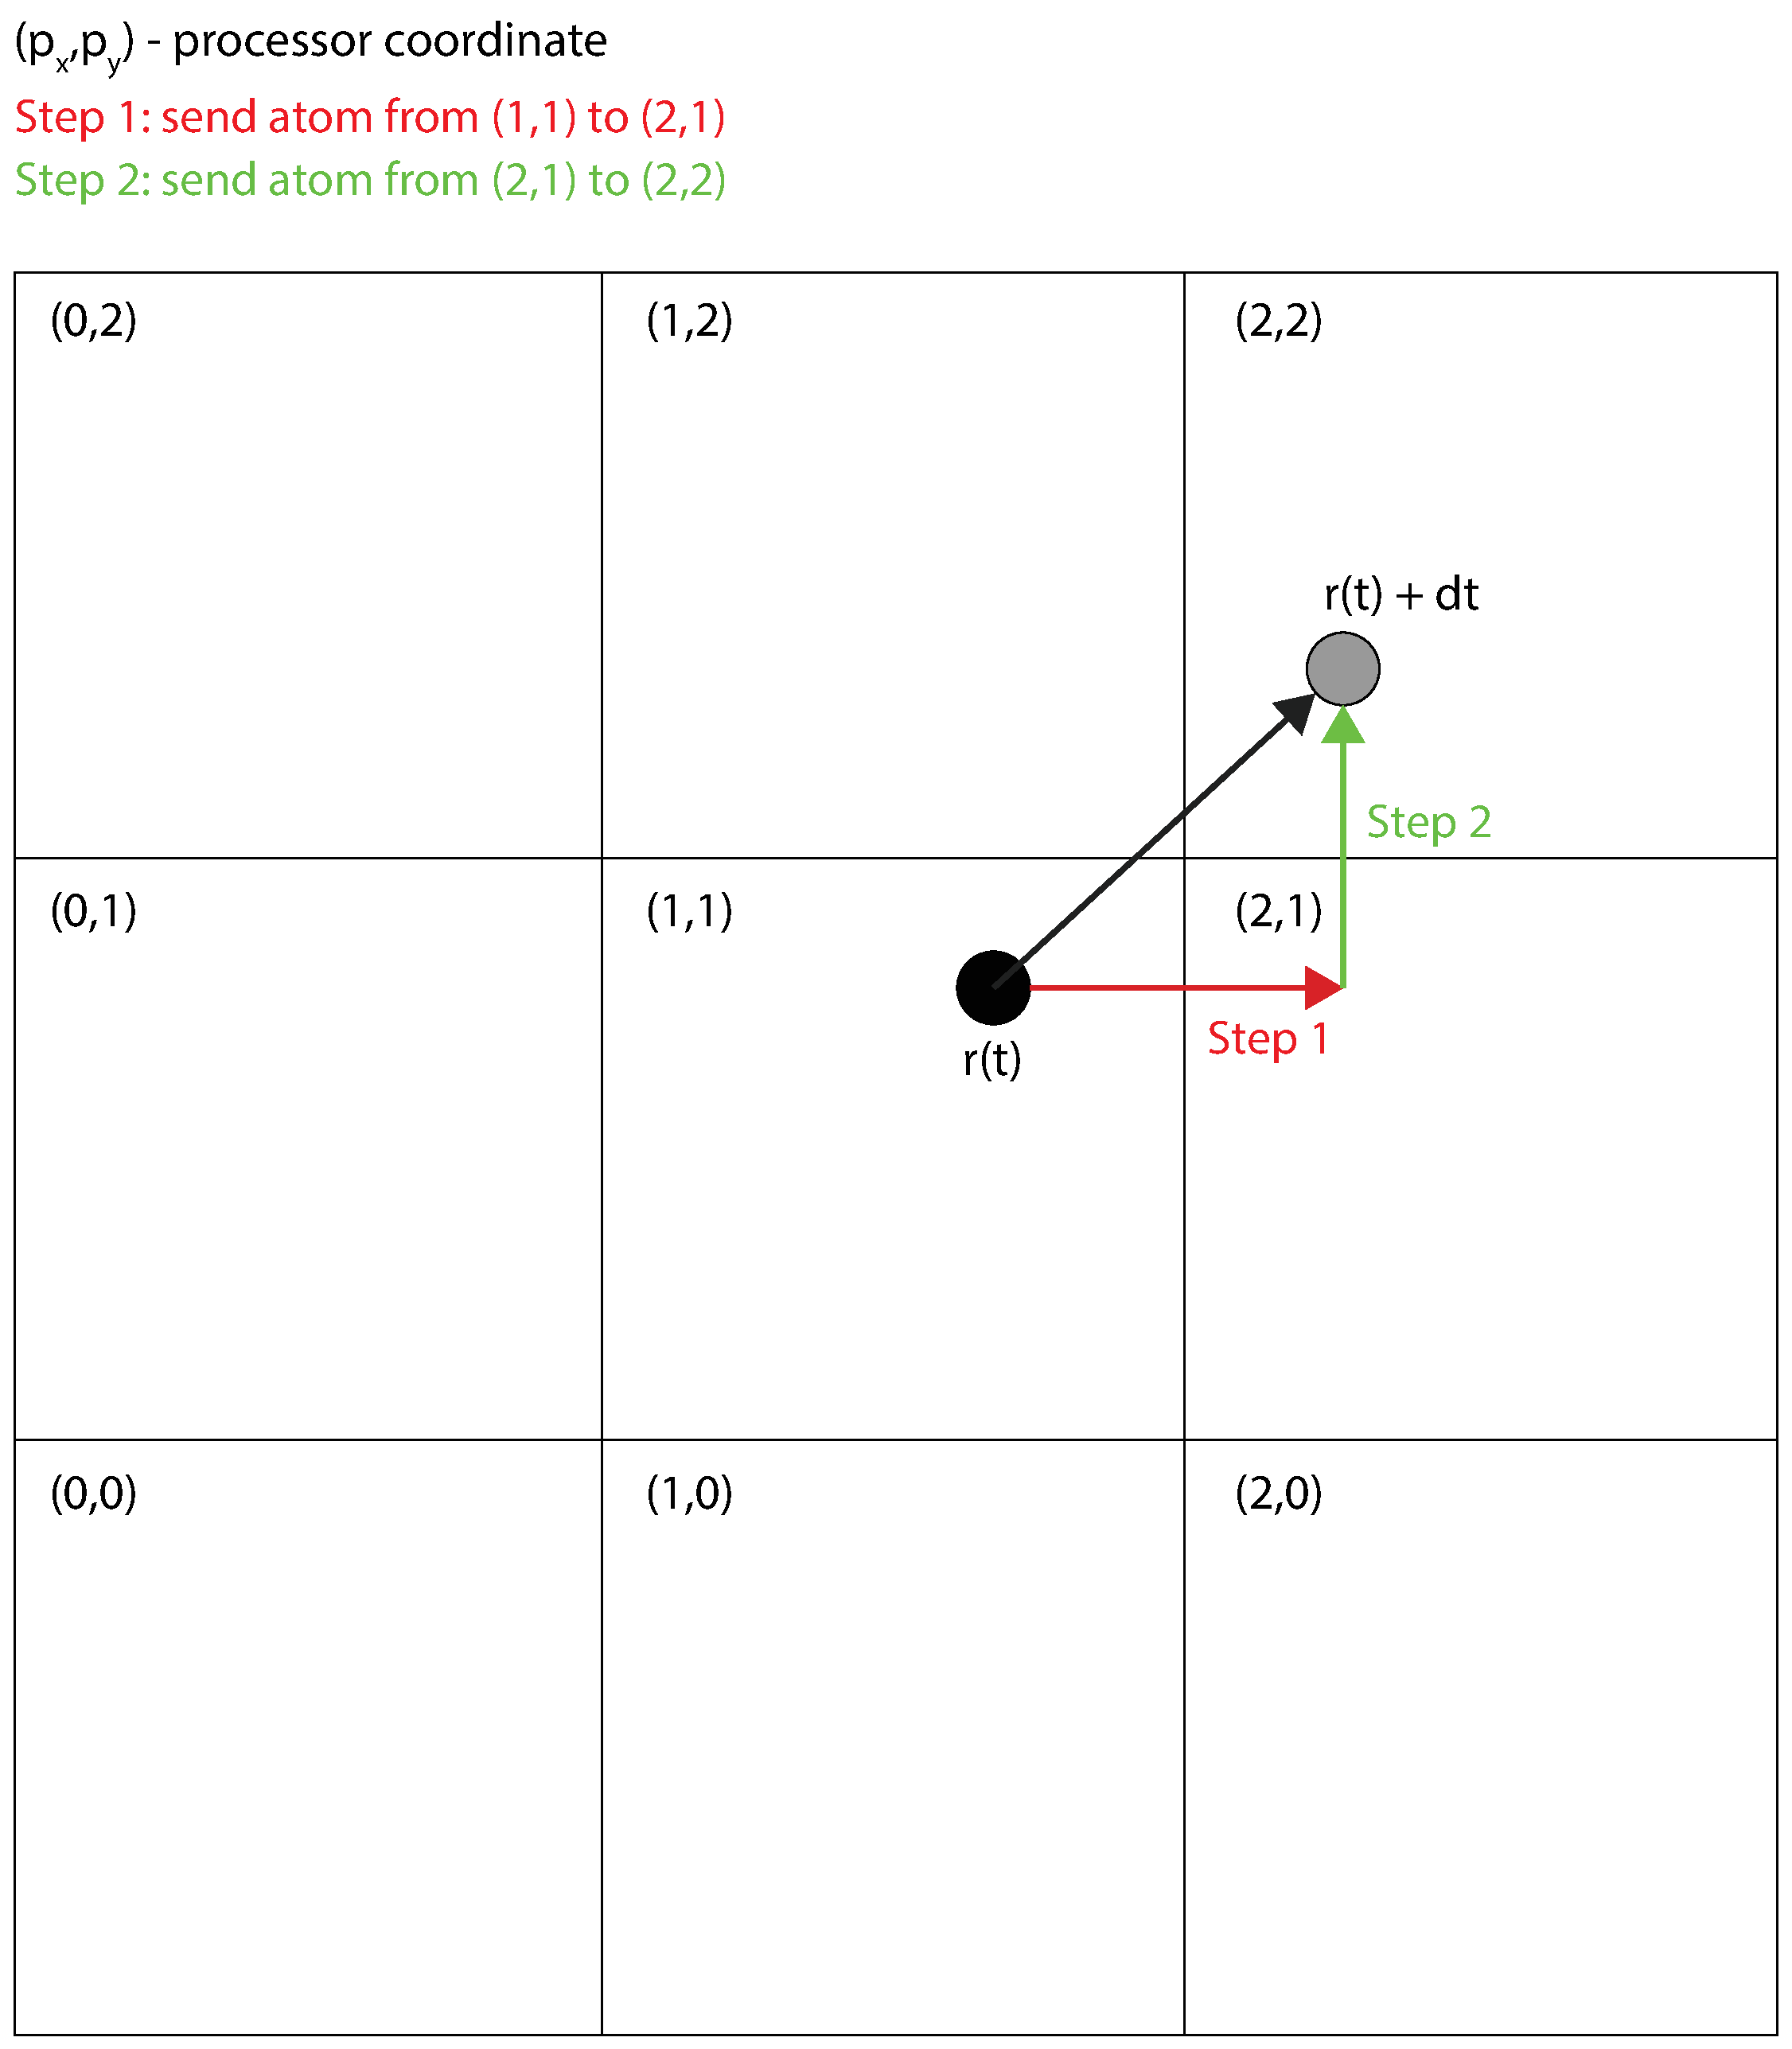
\includegraphics[width=0.7\textwidth, trim=0cm 0cm 0cm 0cm, clip]{MD/figures/parallelization_facet_technique.eps}
\end{center}
\caption{The middle node (1,1) has 8 neighbours it needs to communicate with. Each node only needs to communicate with its nearest neighbours (4 in two dimensions, 6 in three dimensions), because the nearest neighbours can work as intermediate information carriers. An atom moving from processor (1,1) to (2,2) will in step 1 be sent to (2,1), then in step 2 be sent to (2,2).}
\label{fig:md_parallelization_facet_technique}
\end{figure}
We only need to know about the 6 nearest neighbors on each processor. We notice a neat detail here, periodic boundary conditions are automatically taken care of. If we again look at figure \ref{fig:md_parallelization_2}, we have 4 processors in the $x$-direction. The processor to the \textit{right} of $(3,0,1)$ is $(0,0,1)$ if we use periodic boundary conditions. But since we use the local coordinates on each processor, when an atom moves to another processor, its coordinates must be \textit{shifted} so its has correct local coordinates on the new processor. Each processor has one \textit{shift vector} per neighbor, containing the transformation it needs to apply on the atom's coordinates before it moved. If the atom moved through the system boundary (periodic boundary conditions), the shift vector must of course reflect this. 